
% This LaTeX was auto-generated from MATLAB code.
% To make changes, update the MATLAB code and republish this document.

\documentclass{article}
\usepackage{graphicx}
\usepackage{color}

\sloppy
\definecolor{lightgray}{gray}{0.5}
\setlength{\parindent}{0pt}

\begin{document}

    
    
\section*{}


\subsection*{Contents}

\begin{itemize}
\setlength{\itemsep}{-1ex}
   \item Setup Necessary Constants
   \item Loop Through Assigned Datasets and Load Data
   \item calculate deflection for Case 1
   \item calculate Case 2 load position by taking moments about the single load
\end{itemize}


\subsection*{Setup Necessary Constants}

\begin{verbatim}
%clear previous variables
clear all;

%metric conversion factors
g1=32.174;      %acceleration of gravity in ft/sec
g2=9.81;        %acceleration of gravity in m/sec
slug=14.5939;   %kilograms in a slug
newton=4.4482;  %newtons in a pound
meter=0.0254;   %meters in an inch

%dimensions of the truss
l=0.250;         %length of one truss element in meters
L=l*16;            %length of the truss in meters
d=9.525/1000;   %diameter of truss elements in meters
t=1.587/1000;   %thickness of truss elements in meters
E=69.5*10^9;    %elastic modulus in Pa
r_2=d/2;        %outer radius
r_1=r_2-t;      %inner radius
A=(pi*r_2^2)-(pi*r_1^2);                %area of a bar in m^2
I=4*((pi/4)*(r_2^4-r_1^4)+(A*(l/2)^2));  %area moment of inertia in m^4

loadcase = [1 2 3]; %three load cases
dataset = [4 6 4];  %our assigned datasets
x = (0:25:300);      %x array to evaluate polyfit lines
\end{verbatim}


\subsection*{Loop Through Assigned Datasets and Load Data}

\begin{verbatim}
for i = 1:3
    %construct a string that is the file name of each dataset
    filename = "Case " + string(loadcase(i)) + " - " + string(dataset(i));
    %construct a name for that struct field (using struct naming rules
    %which are different from file naming rules)
    %struct is formatted data.Case_x_y where x is load case # and y is
    %assigned dataset NOTE CASE SENSITIVE
    dataname = "Case_" + string(loadcase(i)) + "_" + string(dataset(i));
    %read data into struct using readmatrix
    data.(dataname)=readmatrix(filename);
    %this loop parses out the different loadings
    for j = 1:length(data.(dataname))/10
        %extract ten values at a time for each loading
        data.(dataname + "_" + string(j))=data.(dataname)(1+(10*(j-1)):10+(10*(j-1)),:);
        %take the mean of each set of ten values and store in a new struct
        %called meandata.  Uses the same naming convention as the data
        %struct
        meandata.(dataname)(j,:)=mean(data.(dataname + "_" + string(j)));
        %convert the meandata to metric while leaving the original data in
        %imperial
        meandata.(dataname)(j,1)=(((meandata.(dataname)(j,1))./g1).*slug).*g2;
        meandata.(dataname)(j,2:5)=meandata.(dataname)(j,2:5).*newton;
        meandata.(dataname)(j,6)=meandata.(dataname)(j,6).*meter;
    end
    %now we convert the inline load cell to tension loadings
    calibration = meandata.(dataname)(1,5);
    meandata.(dataname)(:,7)=-(calibration-meandata.(dataname)(:,5));

    %polyfit lines to each load cell, the inline cell, and displacement
    [p1,S1]=polyfit(meandata.(dataname)(:,1),meandata.(dataname)(:,2),1);
    [p2,S2]=polyfit(meandata.(dataname)(:,1),meandata.(dataname)(:,3),1);
    [p3,S3]=polyfit(meandata.(dataname)(:,1),meandata.(dataname)(:,4),1);
    [p4,S4]=polyfit(meandata.(dataname)(:,1),meandata.(dataname)(:,6),1);
    [p5,S5]=polyfit(meandata.(dataname)(:,1),meandata.(dataname)(:,7),1);
    [p6,S6]=polyfit(meandata.(dataname)(:,1),(meandata.(dataname)(:,2)+meandata.(dataname)(:,3)),1);
    fitlines.(dataname)(:,1)=x;
    [fitlines.(dataname)(:,2),fitlines.(dataname)(:,3)]=polyval(p1,x,S1);
    [fitlines.(dataname)(:,4),fitlines.(dataname)(:,5)]=polyval(p2,x,S2);
    [fitlines.(dataname)(:,6),fitlines.(dataname)(:,7)]=polyval(p3,x,S3);
    [fitlines.(dataname)(:,8),fitlines.(dataname)(:,9)]=polyval(p4,x,S4);
    [fitlines.(dataname)(:,10),fitlines.(dataname)(:,11)]=polyval(p5,x,S5);
    [fitlines.(dataname)(:,12),fitlines.(dataname)(:,13)]=polyval(p6,x,S6);
end
\end{verbatim}


\subsection*{calculate deflection for Case 1}

\begin{verbatim}
F_A=meandata.Case_1_4(:,4); %extract relevant data

%calculate deflection for Case 1 at point L/2
coeff_1=1/(E*I);
coeff_2=F_A./6;
coeff_3=(F_A*L^2)./8;
deflection_1=coeff_1.*((coeff_2.*(L/2).^3)-(coeff_3.*(L/2)));

%calculate deflection for Case 2 at point L/2 using d=2.25 m
F_B=meandata.Case_2_6(:,2)+meandata.Case_2_6(:,3);
coeff_2=F_B./6;
coeff_3=(F_B.*81.*L^2)./256;
deflection_2=coeff_1.*((coeff_2.*(L/2).^3)-(coeff_3.*(L/2)));

%check moment eqn by applying to Case 1
F_A=meandata.Case_1_4(:,4);
P=meandata.Case_1_4(:,1);
pos1_1= L.*(1-(F_A./P));
F_B=meandata.Case_1_4(:,2)+meandata.Case_1_4(:,3);
pos2_1= L.*(1-(F_B./P));
pos1_1mean=mean(pos1_1(2:9));
pos2_1mean=mean(pos2_1(2:9));
\end{verbatim}


\subsection*{calculate Case 2 load position by taking moments about the single load}

\begin{verbatim}
%cell
F_A=meandata.Case_2_6(:,4);
P=meandata.Case_2_6(:,1);
pos1_2= L.*(1-(F_A./P));
F_B=meandata.Case_2_6(:,2)+meandata.Case_2_6(:,3);
pos2_2= L.*(1-(F_B./P));
pos1_2mean=mean(pos1_2(2:10));
pos2_2mean=mean(pos2_2(2:10));


%plotting
grid on;
% figure (1);
% hold on;
% scatter(meandata.Case_1_4(:,1),meandata.Case_1_4(:,4),15,'r','filled');
% plot(fitlines.Case_1_4(:,1),fitlines.Case_1_4(:,6),'red');
% scatter(meandata.Case_2_6(:,1),meandata.Case_2_6(:,4),15,'b','filled');
% plot(fitlines.Case_2_6(:,1),fitlines.Case_2_6(:,6),'blue');
% scatter(meandata.Case_3_4(:,1),meandata.Case_3_4(:,4),15,'k','filled');
% plot(fitlines.Case_3_4(:,1),fitlines.Case_3_4(:,6),'black');
% title ("Load Cell F0 (Single)");
% xlabel ("Total Load Weight in Newtons (N)");
% ylabel ("Measured Reaction Force at F0");
% legend("Case 1 Dataset 4","Case 1 Dataset 4 Fit Line","Case 2 Dataset 6",...
%     "Case 2 Dataset 6 Fit Line", "Case 3 Dataset 4",...
%     "Case 3 Dataset 4 Fit Line",'location','southeast');
% hold off;
%
% figure (2);
% hold on;
% scatter(meandata.Case_1_4(:,1),meandata.Case_1_4(:,2),15,'r','filled');
% plot(fitlines.Case_1_4(:,1),fitlines.Case_1_4(:,2),'red');
% scatter(meandata.Case_2_6(:,1),meandata.Case_2_6(:,2),15,'b','filled');
% plot(fitlines.Case_2_6(:,1),fitlines.Case_2_6(:,2),'blue');
% scatter(meandata.Case_3_4(:,1),meandata.Case_3_4(:,2),15,'k','filled');
% plot(fitlines.Case_3_4(:,1),fitlines.Case_3_4(:,2),'black');
% title ("Load Cell F1 (Double)");
% xlabel ("Total Load Weight in Newtons (N)");
% ylabel ("Measured Reaction Force at F1");
% legend("Case 1 Dataset 4","Case 1 Dataset 4 Fit Line","Case 2 Dataset 6",...
%     "Case 2 Dataset 6 Fit Line", "Case 3 Dataset 4",...
%     "Case 3 Dataset 4 Fit Line",'location','southeast');
% hold off;
%
% figure (3);
% hold on;
% scatter(meandata.Case_1_4(:,1),meandata.Case_1_4(:,3),15,'r','filled');
% plot(fitlines.Case_1_4(:,1),fitlines.Case_1_4(:,4),'red');
% scatter(meandata.Case_2_6(:,1),meandata.Case_2_6(:,3),15,'b','filled');
% plot(fitlines.Case_2_6(:,1),fitlines.Case_2_6(:,4),'blue');
% scatter(meandata.Case_3_4(:,1),meandata.Case_3_4(:,3),15,'k','filled');
% plot(fitlines.Case_3_4(:,1),fitlines.Case_3_4(:,4),'black');
% title ("Load Cell F2 (Double)");
% xlabel ("Total Load Weight in Newtons (N)");
% ylabel ("Measured Reaction Force at F2");
% legend("Case 1 Dataset 4","Case 1 Dataset 4 Fit Line","Case 2 Dataset 6",...
%     "Case 2 Dataset 6 Fit Line", "Case 3 Dataset 4",...
%     "Case 3 Dataset 4 Fit Line",'location','southeast');
% hold off;
%
% figure (4);
% hold on;
% g1=scatter(meandata.Case_1_4(:,1),meandata.Case_1_4(:,7),15,'r','filled');
% g2=plot(fitlines.Case_1_4(:,1),fitlines.Case_1_4(:,10),'red');
% g3=plot(fitlines.Case_1_4(:,1),(fitlines.Case_1_4(:,10)-2*fitlines.Case_1_4(:,11)),'red--');
% g4=plot(fitlines.Case_1_4(:,1),(fitlines.Case_1_4(:,10)+2*fitlines.Case_1_4(:,11)),'red--');
% g5=scatter(meandata.Case_2_6(:,1),meandata.Case_2_6(:,7),15,'b','filled');
% g6=plot(fitlines.Case_2_6(:,1),fitlines.Case_2_6(:,10),'blue');
% g7=plot(fitlines.Case_2_6(:,1),(fitlines.Case_2_6(:,10)-2*fitlines.Case_2_6(:,11)),'blue--');
% g8=plot(fitlines.Case_2_6(:,1),(fitlines.Case_2_6(:,10)+2*fitlines.Case_2_6(:,11)),'blue--');
% g9=scatter(meandata.Case_3_4(:,1),meandata.Case_3_4(:,7),15,'k','filled');
% g10=plot(fitlines.Case_3_4(:,1),fitlines.Case_3_4(:,10),'black');
% g11=plot(fitlines.Case_3_4(:,1),(fitlines.Case_3_4(:,10)-2*fitlines.Case_3_4(:,11)),'black--');
% g12=plot(fitlines.Case_3_4(:,1),(fitlines.Case_3_4(:,10)+2*fitlines.Case_3_4(:,11)),'black--');
% title ("Inline Load Cell Tension Force");
% xlabel ("Total Load Weight in Newtons (N)");
% ylabel ("Measured Tension Force at Bottom Center");
%  legend([g1,g2,g5,g6,g9,g10],"Case 1 Dataset 4","Case 1-4 Fit Line w/95% Interval","Case 2 Dataset 6",...
%      "Case 2-6 Fit Line w/95% Interval", "Case 3 Dataset 4",...
%      "Case 3-4 Fit Line w/95% Interval",'location','southeast');
%  legend('boxoff');
% hold off;
% %
% figure (5);
% hold on;
% g1=scatter(meandata.Case_1_4(:,1),meandata.Case_1_4(:,6),15,'r','filled');
% g2=plot(fitlines.Case_1_4(:,1),fitlines.Case_1_4(:,8),'red');
% g3=plot(fitlines.Case_1_4(:,1),(fitlines.Case_1_4(:,8)-2*fitlines.Case_1_4(:,9)),'red--');
% g4=plot(fitlines.Case_1_4(:,1),(fitlines.Case_1_4(:,8)+2*fitlines.Case_1_4(:,9)),'red--');
% g5=scatter(meandata.Case_2_6(:,1),meandata.Case_2_6(:,6),15,'b','filled');
% g6=plot(fitlines.Case_2_6(:,1),fitlines.Case_2_6(:,8),'blue');
% g7=plot(fitlines.Case_2_6(:,1),(fitlines.Case_2_6(:,8)-2*fitlines.Case_2_6(:,9)),'blue--');
% g8=plot(fitlines.Case_2_6(:,1),(fitlines.Case_2_6(:,8)+2*fitlines.Case_2_6(:,9)),'blue--');
% g9=scatter(meandata.Case_3_4(:,1),meandata.Case_3_4(:,6),15,'k','filled');
% g10=plot(fitlines.Case_3_4(:,1),fitlines.Case_3_4(:,8),'black');
% g11=plot(fitlines.Case_3_4(:,1),(fitlines.Case_3_4(:,8)-2*fitlines.Case_3_4(:,9)),'black--');
% g12=plot(fitlines.Case_3_4(:,1),(fitlines.Case_3_4(:,8)+2*fitlines.Case_3_4(:,9)),'black--');
% title ("Displacement at Center");
% xlabel ("Total Load Weight in Newtons (N)");
% ylabel ("Measured Displacement in Meters");
% legend([g1,g2,g5,g6,g9,g10],"Case 1 Dataset 4","Case 1 Dataset 4 Fit Line","Case 2 Dataset 6",...
%     "Case 2 Dataset 6 Fit Line", "Case 3 Dataset 4",...
%     "Case 3 Dataset 4 Fit Line",'location','southeast');
% legend('boxoff');
% hold off;
%
% figure (6);
% hold on;
% scatter(meandata.Case_1_4(:,1),(meandata.Case_1_4(:,2)+meandata.Case_1_4(:,3)),15,'r','filled');
% plot(fitlines.Case_1_4(:,1),fitlines.Case_1_4(:,12),'red');
% scatter(meandata.Case_2_6(:,1),(meandata.Case_2_6(:,2)+meandata.Case_2_6(:,3)),15,'b','filled');
% plot(fitlines.Case_2_6(:,1),fitlines.Case_2_6(:,12),'blue');
% scatter(meandata.Case_3_4(:,1),(meandata.Case_3_4(:,2)+meandata.Case_3_4(:,3)),15,'k','filled');
% plot(fitlines.Case_3_4(:,1),fitlines.Case_3_4(:,12),'black');
% title ("Combined Load Cells F1 & F2");
% xlabel ("Total Load Weight in Newtons (N)");
% ylabel ("Measured Reaction Force in Newtons");
% legend("Case 1 Dataset 4","Case 2 Dataset 6",...
%     "Case 2 Dataset 6 Fit Line", "Case 3 Dataset 4",...
%     "Case 3 Dataset 4 Fit Line",'location','southeast');
% hold off;

% figure (7);
% hold on;
% g1=scatter(meandata.Case_1_4(:,1),meandata.Case_1_4(:,4),15,'r','filled');
% g2=plot(fitlines.Case_1_4(:,1),fitlines.Case_1_4(:,6),'red');
% g3=plot(fitlines.Case_1_4(:,1),(fitlines.Case_1_4(:,6)-2*fitlines.Case_1_4(:,7)),'red--');
% g4=plot(fitlines.Case_1_4(:,1),(fitlines.Case_1_4(:,6)+2*fitlines.Case_1_4(:,7)),'red--');
% g5=scatter(meandata.Case_1_4(:,1),meandata.Case_1_4(:,2),15,'b','filled');
% g6=plot(fitlines.Case_1_4(:,1),fitlines.Case_1_4(:,2),'blue');
% g7=plot(fitlines.Case_1_4(:,1),(fitlines.Case_1_4(:,2)-2*fitlines.Case_1_4(:,3)),'blue--');
% g8=plot(fitlines.Case_1_4(:,1),(fitlines.Case_1_4(:,2)+2*fitlines.Case_1_4(:,3)),'blue--');
% g9=scatter(meandata.Case_1_4(:,1),meandata.Case_1_4(:,3),15,'k','filled');
% g10=plot(fitlines.Case_1_4(:,1),fitlines.Case_1_4(:,4),'black');
% g11=plot(fitlines.Case_1_4(:,1),(fitlines.Case_1_4(:,4)-2*fitlines.Case_1_4(:,5)),'black--');
% g12=plot(fitlines.Case_1_4(:,1),(fitlines.Case_1_4(:,4)+2*fitlines.Case_1_4(:,5)),'black--');
% g13=scatter(meandata.Case_1_4(:,1),(meandata.Case_1_4(:,2)+meandata.Case_1_4(:,3)),15,'m','filled');
% g14=plot(fitlines.Case_1_4(:,1),fitlines.Case_1_4(:,12),'magenta');
% g15=plot(fitlines.Case_1_4(:,1),(fitlines.Case_1_4(:,12)-2*fitlines.Case_1_4(:,13)),'magenta--');
% g16=plot(fitlines.Case_1_4(:,1),(fitlines.Case_1_4(:,12)+2*fitlines.Case_1_4(:,13)),'magenta--');
% title ("Load Case 1 Reaction Forces");
% xlabel ("Total Load Weight in Newtons (N)");
% ylabel ("Measured Reaction Forces in Newtons (N)");
% legend([g1 g2 g5 g6 g9 g10 g13 g14],"Load Cell F2","F2 Fit Line w/95% Interval","Load Cell F0",...
%     "F0 Fit Line w/95% Fit Line", "Load Cell F1",...
%     "F1 Fit Line w/95% Interval","Load Cells F0+F1", "F0+F1 Fit Line w/95% Interval",...
%     'location','southeast');
% legend('boxoff');
% ylim([-40,160]);
% hold off;
%
% figure (8);
% hold on;
% g1=scatter(meandata.Case_2_6(:,1),meandata.Case_2_6(:,4),15,'r','filled');
% g2=plot(fitlines.Case_2_6(:,1),fitlines.Case_2_6(:,6),'red');
% g3=plot(fitlines.Case_2_6(:,1),(fitlines.Case_2_6(:,6)-2*fitlines.Case_2_6(:,7)),'red--');
% g4=plot(fitlines.Case_2_6(:,1),(fitlines.Case_2_6(:,6)+2*fitlines.Case_2_6(:,7)),'red--');
% g5=scatter(meandata.Case_2_6(:,1),meandata.Case_2_6(:,2),15,'b','filled');
% g6=plot(fitlines.Case_2_6(:,1),fitlines.Case_2_6(:,2),'blue');
% g7=plot(fitlines.Case_2_6(:,1),(fitlines.Case_2_6(:,2)-2*fitlines.Case_2_6(:,3)),'blue--');
% g8=plot(fitlines.Case_2_6(:,1),(fitlines.Case_2_6(:,2)+2*fitlines.Case_2_6(:,3)),'blue--');
% g9=scatter(meandata.Case_2_6(:,1),meandata.Case_2_6(:,3),15,'k','filled');
% g10=plot(fitlines.Case_2_6(:,1),fitlines.Case_2_6(:,4),'black');
% g11=plot(fitlines.Case_2_6(:,1),(fitlines.Case_2_6(:,4)-2*fitlines.Case_2_6(:,5)),'black--');
% g12=plot(fitlines.Case_2_6(:,1),(fitlines.Case_2_6(:,4)+2*fitlines.Case_2_6(:,5)),'black--');
% g13=scatter(meandata.Case_2_6(:,1),(meandata.Case_2_6(:,2)+meandata.Case_2_6(:,3)),15,'m','filled');
% g14=plot(fitlines.Case_2_6(:,1),fitlines.Case_2_6(:,12),'magenta');
% g15=plot(fitlines.Case_2_6(:,1),(fitlines.Case_2_6(:,12)-2*fitlines.Case_2_6(:,13)),'magenta--');
% g16=plot(fitlines.Case_2_6(:,1),(fitlines.Case_2_6(:,12)+2*fitlines.Case_2_6(:,13)),'magenta--');
% title ("Load Case 2 Reaction Forces");
% xlabel ("Total Load Weight in Newtons (N)");
% ylabel ("Measured Reaction Forces in Newtons (N)");
% legend([g1 g2 g5 g6 g9 g10 g13 g14],"Load Cell F2","F2 Fit Line w/95% Interval","Load Cell F0",...
%     "F0 Fit Line w/95% Fit Line", "Load Cell F1",...
%     "F1 Fit Line w/95% Interval","Load Cells F0+F1", "F0+F1 Fit Line w/95% Interval",...
%     'location','southeast');
% legend('boxoff');
% ylim([-40,160]);
% hold off;
%
% figure (9);
% hold on;
% g1=scatter(meandata.Case_3_4(:,1),meandata.Case_3_4(:,4),15,'r','filled');
% g2=plot(fitlines.Case_3_4(:,1),fitlines.Case_3_4(:,6),'red');
% g3=plot(fitlines.Case_3_4(:,1),(fitlines.Case_3_4(:,6)-2*fitlines.Case_3_4(:,7)),'red--');
% g4=plot(fitlines.Case_3_4(:,1),(fitlines.Case_3_4(:,6)+2*fitlines.Case_3_4(:,7)),'red--');
% g5=scatter(meandata.Case_3_4(:,1),meandata.Case_3_4(:,2),15,'b','filled');
% g6=plot(fitlines.Case_3_4(:,1),fitlines.Case_3_4(:,2),'blue');
% g7=plot(fitlines.Case_3_4(:,1),(fitlines.Case_3_4(:,2)-2*fitlines.Case_3_4(:,3)),'blue--');
% g8=plot(fitlines.Case_3_4(:,1),(fitlines.Case_3_4(:,2)+2*fitlines.Case_3_4(:,3)),'blue--');
% g9=scatter(meandata.Case_3_4(:,1),meandata.Case_3_4(:,3),15,'k','filled');
% g10=plot(fitlines.Case_3_4(:,1),fitlines.Case_3_4(:,4),'black');
% g11=plot(fitlines.Case_3_4(:,1),(fitlines.Case_3_4(:,4)-2*fitlines.Case_3_4(:,5)),'black--');
% g12=plot(fitlines.Case_3_4(:,1),(fitlines.Case_3_4(:,4)+2*fitlines.Case_3_4(:,5)),'black--');
% g13=scatter(meandata.Case_3_4(:,1),(meandata.Case_3_4(:,2)+meandata.Case_3_4(:,3)),15,'m','filled');
% g14=plot(fitlines.Case_3_4(:,1),fitlines.Case_3_4(:,12),'magenta');
% g15=plot(fitlines.Case_3_4(:,1),(fitlines.Case_3_4(:,12)-2*fitlines.Case_3_4(:,13)),'magenta--');
% g16=plot(fitlines.Case_3_4(:,1),(fitlines.Case_3_4(:,12)+2*fitlines.Case_3_4(:,13)),'magenta--');
% title ("Load Case 3 Reaction Forces");
% xlabel ("Total Load Weight in Newtons (N)");
% ylabel ("Measured Reaction Forces in Newtons (N)");
% legend([g1 g2 g5 g6 g9 g10 g13 g14],"Load Cell F2","F2 Fit Line w/95% Interval","Load Cell F0",...
%     "F0 Fit Line w/95% Fit Line", "Load Cell F1",...
%     "F1 Fit Line w/95% Interval","Load Cells F0+F1", "F0+F1 Fit Line w/95% Interval",...
%     'location','southeast');
% legend('boxoff');
% ylim([-40,160]);
% hold off;
%
% figure (10);
% hold on;
%
% g5=scatter(meandata.Case_2_6(:,1),meandata.Case_2_6(:,6),15,'b','filled');
% g9=scatter(meandata.Case_2_6(:,1),-deflection_2,15,'k','filled');
% g6=plot(fitlines.Case_2_6(:,1),fitlines.Case_2_6(:,8),'blue');
% g7=plot(fitlines.Case_2_6(:,1),(fitlines.Case_2_6(:,8)-2*fitlines.Case_2_6(:,9)),'blue--');
% g8=plot(fitlines.Case_2_6(:,1),(fitlines.Case_2_6(:,8)+2*fitlines.Case_2_6(:,9)),'blue--');
% title ("Displacement at Center Experimental vs. Model, Case 2");
% xlabel ("Total Load Weight in Newtons (N)");
% ylabel ("Measured Displacement in Meters");
% legend("Case 2 Deflection (Exp) w/Fit Line","Case 2 Deflection (Model)",...
%     'location','southeast');
% legend('boxoff');
% hold off;
\end{verbatim}

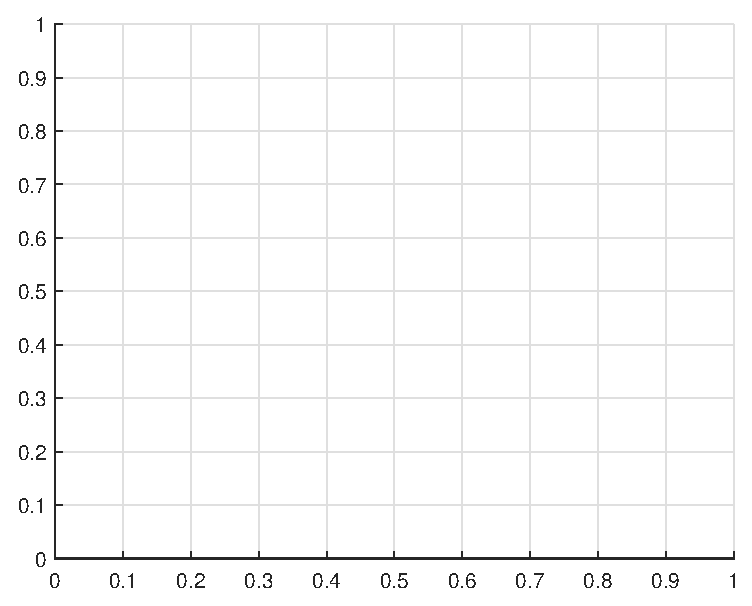
\includegraphics [width=4in]{Lab1data_01.eps}



\end{document}

